\documentclass[12pt]{report}
\usepackage[top=1in, bottom=1in, left=1.5in, right=1in]{geometry}
\usepackage{helvet}
\renewcommand{\familydefault}{\sfdefault}             		
\usepackage{graphicx}
\usepackage{subcaption}
\usepackage{pdfpages}
\usepackage{booktabs}
\usepackage{listings}
\lstset{
    frame=single,
    breaklines=true,
    showstringspaces=false,
    basicstyle=\tiny,
}
\usepackage{latexsym}
\usepackage{array}
\usepackage{amsmath}					
\usepackage[backend=biber]{biblatex}
\addbibresource{thesis.bib}
\usepackage[utf8]{inputenc}
\usepackage[titletoc]{appendix}
\usepackage{xspace}
\newcommand{\sysname}{\textsc{Soar}\xspace}
\newcommand{\sandboxname}{\sysname-Repy\xspace}


\begin{document}

\includepdf[pages={1-2}]{./cover/titlepage.pdf}
\pagenumbering{roman}
\setcounter{page}{2}
\chapter*{VITA}
\textbf{Xuefeng Huang} received his bachelor degree in information security at Nanjing University of Posts and Telecommunications, China, in 2014. Since September 2014 he entered the Tandon School of Engineering at New York University. His master thesis covers distributed testbed and wireless network measurement. His other research interests include cyber security as well as virtualization. In the past he also worked on program slicing technology as part of the work for his bachelor thesis.
\chapter*{ACKNOWLEDGEMENTS}
This thesis owes its existence to help, support and inspiration of several people. First of all, I would like to express my special thanks of gratitude to my advisor Prof. Justin Cappos for guidance during my research. His support, encouragement and inspiring suggestions have been precious for the development of this thesis content.

I am also indebted to my co-advisor Prof. Albert Rafetseder, who offered his continuous advice and encouragement throughout the course of this thesis. I am so deeply grateful for his help, professionalism and valuable guidance throughout this project and through my entire program of study that I do not have enough words to express my deep and sincere appreciation. 

A big thanks also goes to Seattle Testbed group members, there are not enough words to describe your excellent work. Ajay and Priyam, thanks for helping me test platform. Lois, I am really appreciated for your guidance and helpful feedback. Vlad and Sebastien, thanks for your useful inputs and discussion.    

Last, but not least, I would like to thank my parents for their dedication and the many years of support during my graduate studies that provided the foundation for this work.

It is impossible to acknowledge everyone here. It must suffice to say that this thesis owes a lot to a lot of people.

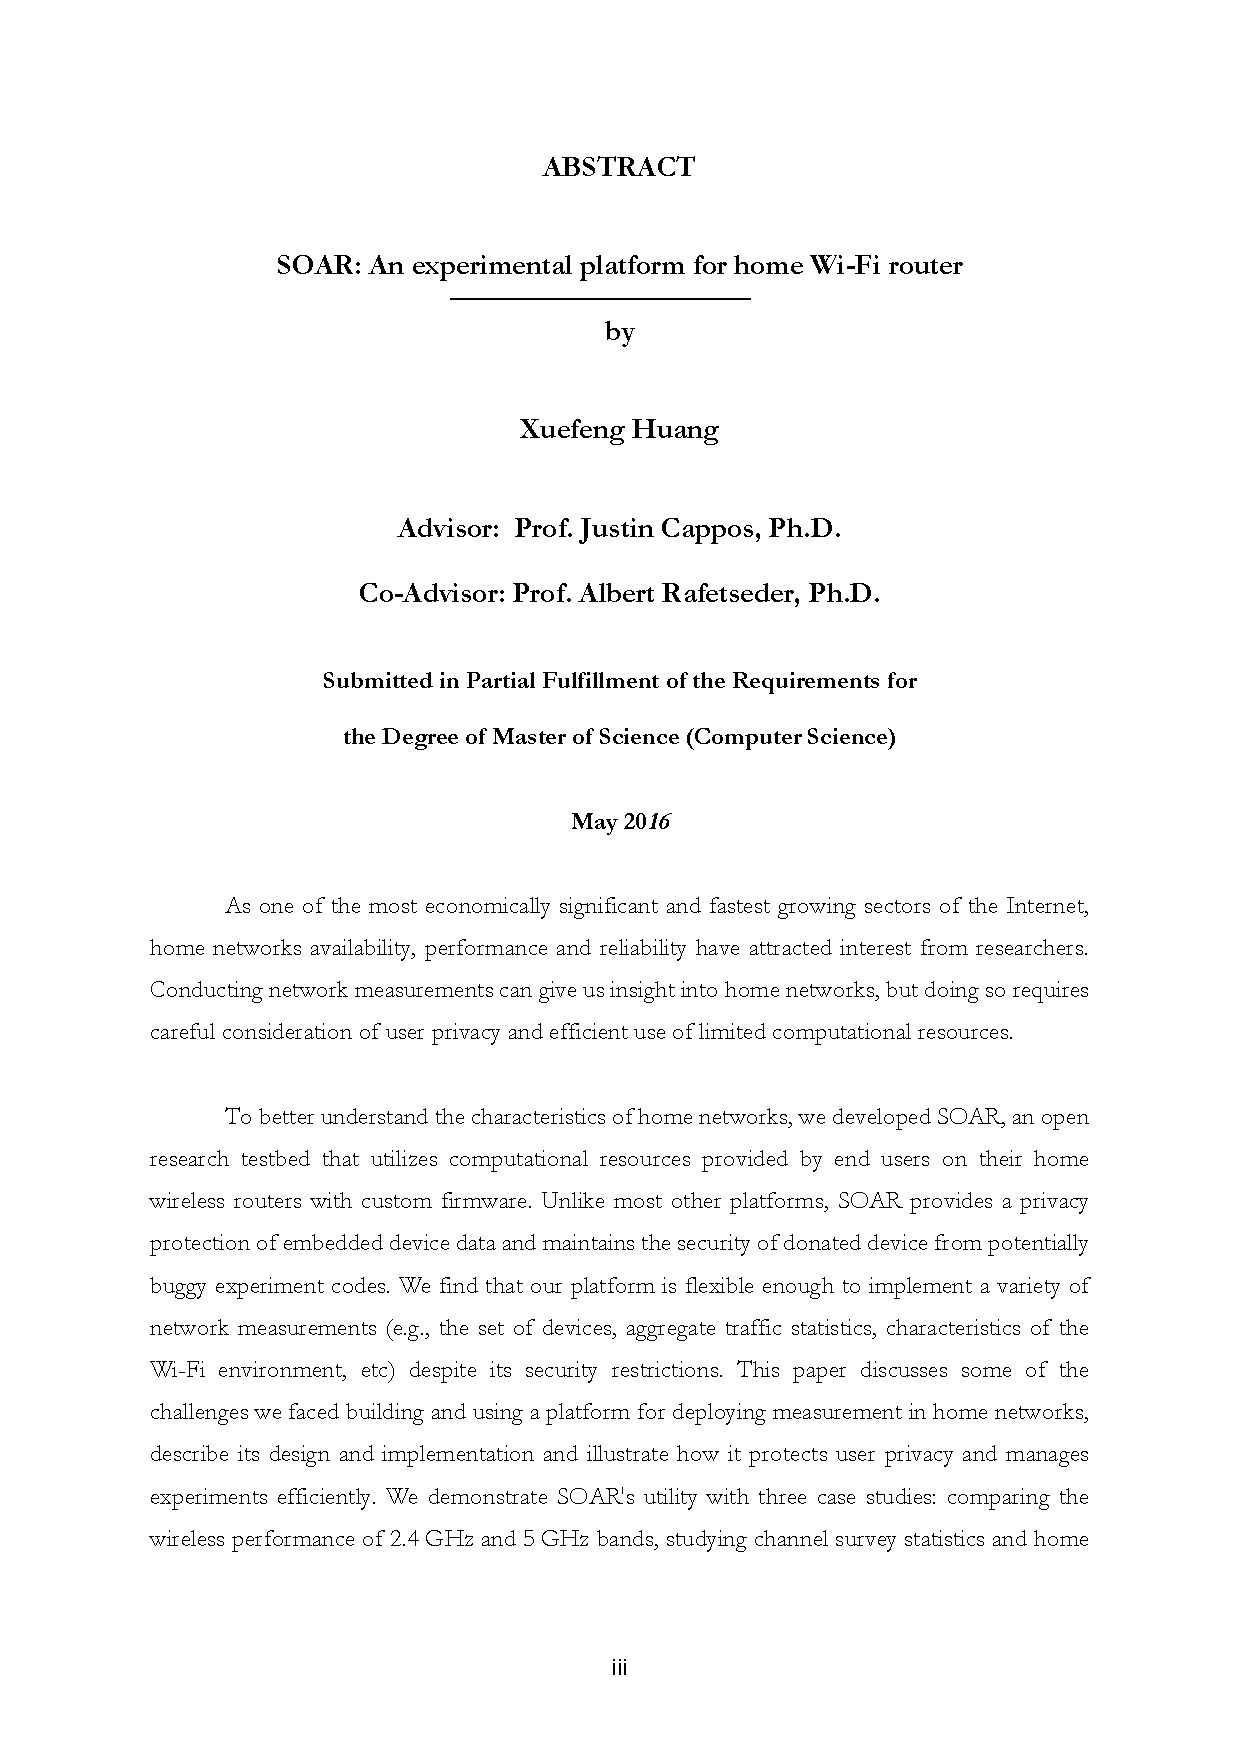
\includepdf[pages={1}]{./cover/ABSTRACT.pdf}
\tableofcontents
\listoffigures
\listoftables
\lstlistoflistings
%\begin{abstract}
As one of the most economically significant and fastest growing sectors of 
the Internet, broadband networks have attracted interest from researchers. 
To better understand broadband networks, we developed Seattle, an open 
research and educational testbed that utilizes computational resources 
provided by end users on their home wireless routers with custom firmware. 
Unlike most other platforms, Seattle provides a privacy protection of 
embedded device data and maintains the security of donated device from 
potentially buggy experiment codes. We find that our platform is flexible 
enough to implement a variety of network measurement despite its security 
restrictions. This paper discusses some of the challenges we faced building 
and using a platform for deploying measurement in home networks, describe 
its design and implementation.
\end{abstract}
\clearpage
%\section{}
%\subsection{}
\pagenumbering{arabic}
\chapter{INTRODUCTION}
\label{sec.introduction}
Broadband Internet access for home use is rapidly evolving. The United States
alone has more than 279 million broadband users. The number of Internet 
users in other regions is even more impressive, with China counting more 
than 641 million~\cite{asia}. Yet, despite its pervasiveness, little is 
known about most home network's availability, performance and reliability. This lack of knowledge hampers progress in a number of important research 
areas, from ISP performance to large-scale
topology mapping and wireless network utilization. Researchers, policymakers 
and Internet Service Providers (ISPs) are also eager to learn more about 
emerging technologies made possible by these networks. ``Smart homes," in 
which devices from thermostats to door locks can be controlled remotely are
 now exciting realities. In 2016, 4 billion new objects (e.g., laptops, 
handhelds, interactive television, wireless based security cameras) will 
become available to consumers~\cite{gartner}. But with the benefits of these 
products also come concerns. For these devices to work, they usually need to 
be connected to a wireless router. If a router is compromised via buggy 
software, it is possible that hackers could unlock not only critical data, 
but also someone's front door. Therefore, as their use grows, understanding 
vulnerabilities in both routers and broadband networks becomes crucial in 
order to prevent these types of attacks.

Due to these challenges, the value of studying home networks for researchers, 
policy makers and ISPs continues to grow. At this point in time studying 
home networks on a large scale has been difficult because network 
technologies, such as network address translators (NATs), present only a 
partial view of the home network to the global Internet. To better understand 
the behavior of networks, a formal study using an experimental platform that 
can gather data from homes is needed to provide visibility into the 
unseen sections of the network. Such a platform should also provide a set of 
programming interfaces to support as wide an array of measurements as 
possible, including factors affecting broadband performance, or data that 
can increase understanding of usage and connectivity in home networks.
Lastly, the platform proposed here must ensure the privacy of the 
user and prevent abuse of his or her device or network resources.

A number of measurement and experimentation platforms have been developed to 
support controlled network experimentation and broadband characterization 
for home networks, including gateway-based platforms~\cite{bajpai2014lessons,
samknows,183951,yiakoumis2014behop} and browser or host-based platforms~\cite{
dhawan2012fathom,kreibich2010netalyzr,sanchez2014measurement}. Host-based 
platforms run as applications on the client side and typically suffer from a 
few limitations (e.g., reflecting the network performance of the host or 
application rather than of the network itself, providing only one-shot 
measurements rather than continuous measurements). A gateway-based platform, 
on the other hand, enables continuous measurements and collects network 
feedbacks from all the WiFi devices in the home networks. However, these 
platforms can not balance the trade-off between functionality and security.
 For instance, the process of vetting BISmark~\cite{183951} experiments for 
researchers is manual, which will be a limiting factor as deployment grows. 
Inspired by these projects, we decided to design a gateway-based platform 
that enables continuous, comprehensive and direct measurements. We also 
designed the platform with user security and privacy as first-order concerns.
 
In this paper, we introduce \sysname, a distributed cloud platform that 
allows researchers to run both active and passive experiments securely from 
a wireless router on a home network. Through a programmable interface on the 
device, the platform enables researchers to deploy a wide range of network 
measurements from a vantage point between the access ISP and the home 
network, as shown in Figure~\ref{figure:design}. Researchers can access and 
compile data on systems worldwide, while preserving the user's privacy, and 
securing the device itself. The information gathered from such studies could 
assist users in evaluating the services they are paying for, researchers in 
understanding the factors impacting performance, and ISPs in finding ways to 
improve their service. Because it is designed for running measurement 
software on a home access point, a platform like \sysname has a number of 
unique strengths and challenges. First, software must be small and easy-to-
deploy because \sysname is deployed on resource-constrained devices. Second, 
\sysname sits on the direct path of real Internet users. Any buggy or 
malicious experiments could be able to disrupt Internet connectivity. Thus 
it must guarantee that a poorly designed experiment can not negatively 
affect a user's Internet connection. Third, it is important to make the 
system robust by providing remote maintenance and updates because of the 
unmanaged complexity of its home network environments. Finally, \sysname 
must provide a rich set of APIs for a variety of network measurements. 

\begin{figure}%[h]
\centering
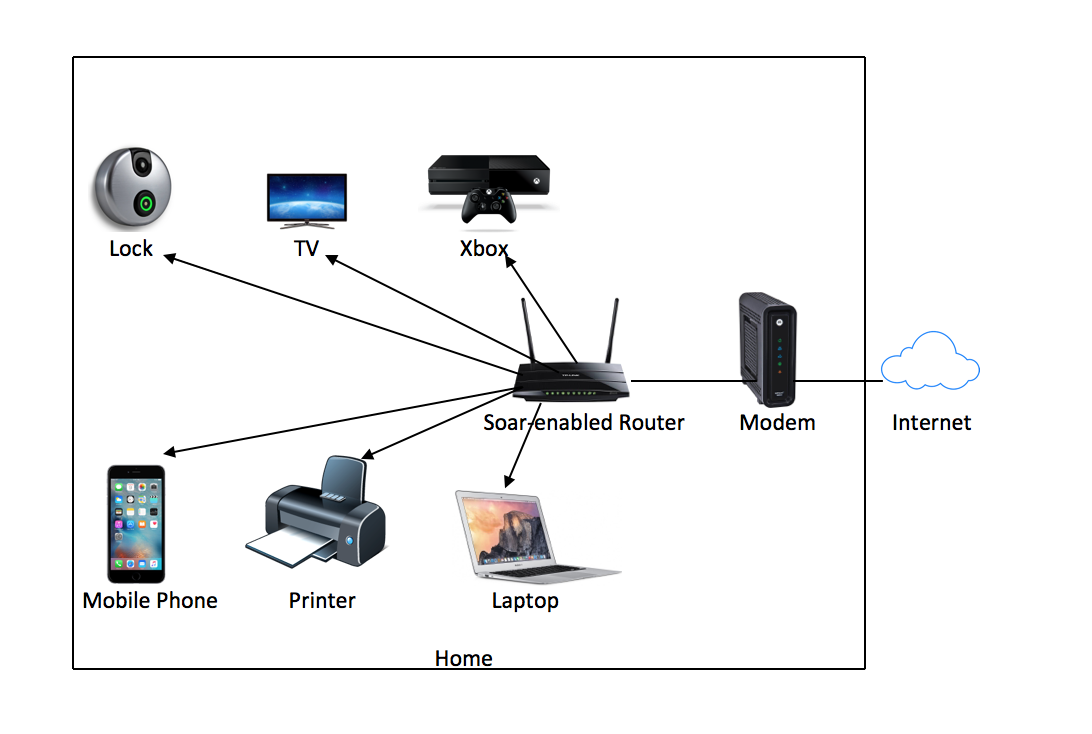
\includegraphics[width=0.8\columnwidth]{figure/home-network.png}
\caption{The \sysname-enabled router sits on the direct path of real 
Internet users. It supports both active and passive network measurements.}
\label{figure:design}
\end{figure}


\sysname is based on Seattle testbed, a community-driven and open-source cloud computing system~\cite{zhuang2013experience,cappos2009seattle}. Compared to computer and mobile device environments, deployment on home wireless routers has more resource limitations, such as restricted computational resources. However, recently we have been able to port Seattle Testbed to OpenWrt, a popular Linux platform for home routers~\cite{openwrt}. Users can build their own \sysname installer (IPK) via a config file we provide using OpenWrt SDK and install it on the device directly. 


\sysname supports standard implementations of useful measurement primitives such as ping, traceroute, network traffic capture, and the like. We extend eight functionalities based on Repy (the core sandbox of Seattle), include 
\texttt{get\_network\_
bytes}, \texttt{get\_network\_packets}, \texttt{get\_network\_interfaces}, \texttt{wifi\_status}, \texttt{scan}, \texttt{get\_
station}, \texttt{ping} and \texttt{traceroute}. This rich set of measurement primitives help researchers to implement a wide range of network measurements, such as mapping Internet paths (via traceroute), studying home network usage patterns and understanding wireless network performance.

\sysname supports a constrained environment of programmable measurements. In order to securely interact with home routers on remote user devices, we use Fence (a non-intrusive mechanism that mediates and limits access to diverse resources using uniform resource control)~\cite{li2015fence} to allocate a fixed percentage of the device's CPU, memory disk, and other resources to one or more VMs. For example, we set the legal times of accessing the \texttt{/proc} file system to prevent DoS attacks using our API calls. To prevent exfiltration of sensitive information from devices, we use security layers to mediate access to the wireless sensor by restricting capability access and reducing the precision of returned data. 


By integrating \sysname into home networks, we get the benefits of a real world deployment while ensuring flexibility to run experiments without compromising home networks. We demonstrate \sysname's utility by implementing both active and passive measurements that together exercise different new API calls. We monitor our lab's network traffic, which is in an office building, from the vantage point of the access point. We report on additional experiences gained using \sysname in three different use cases. We find that there are many factors affecting throughput on 2.4 GHz and 5 GHz band. We also find that most of the access points select non-overlapping channels (e.g., channel 1, 6, 11) to avoid adjacent-channel interference. 


The primary contributions of this study are as follows:
\begin{itemize}
\item We introduce \sysname as a platform for experimentation on home wireless routers that provide a programmable sandboxed environment and dynamic access control mechanism for router security and privacy. Our design ensures experiment code cannot harm the devices of users and reduces the risk of privacy problems through the use of security layers.
\item We implement new research capabilities for home wireless routers by improving on the Seattle sandbox. This rich set of measurement primitives help researchers to implement a wide range of network measurements, such as mapping Internet paths (via traceroute), studying home network usage patterns and understanding wireless network performance.
\item To our knowledge, we are the first wireless router testbed to provide both security and performance isolation using a sandbox environment. 
\end{itemize}


The rest of this thesis is structured as follows: We provide related work and motivation in \S{\ref{sec.relatedwork_motivation}}. In \S{\ref{sec.goals_challenges}}, we point out the goals and challenges of our work. \S{\ref{sec.design}} and \S{\ref{sec.implementation}} describes the design and implementation of \sysname and characterizes our current deployment. Then we present three study cases to illustrate the benefits of an experimental platform that can run on a home wireless router in \S{\ref{sec.evaluation}}. Finally, we discuss our conclusions in \S{\ref{sec.conclusion}}. 
\section{Related Work}
\label{sec.related_work}
Our work shares goals with and builds upon ideas from several prior large-
scale platforms targeting home network research.In the following paragraphs, 
we briefly review related works on network testbed. 
\begin{itemize}
\item \textbf{BISmark} is similar to Seattle in that it is deployed in home 
networks on resource-constrained devices. And currently it is used and 
shared by researchers at nine institutions, including commercial Internet 
service providers, and has enabled studies of access link performance, 
network connectivity, Web page load times, and user behavior and activity. 
However, vetting experiments is challenging. A poorly designed (or controlled
) experiment can cripple a user?s Internet connection. Seattle is supported 
to run arbitrary codes on remote devices without compromising the security 
and privacy of device owners.
\item \textbf{Samknows} has designed and developed its performance tests in 
house, adhering to IETF RFCs where appropriate. All measurements are written 
in C, for performance and portability across a range of hardware platforms. 
But it only supports limited performance measurements. Seattle supports a 
very flexible language for experiment specification based on a restricted 
subset of Python.
\item \textbf{The RIPE Atlas project} is a global network of probes that 
measure Internet connectivity and reachability, providing an unprecedented 
understanding of the state of the Internet in real time. It has deployed 
thousands of probing devices worldwide, but their capabilities are limited 
to simple measurements (e.g., ping, traceroute). Seattle instead provides a 
wide range of capabilities to support complex measurements. 
\item \textbf{Dasu} is a measurement experimentation platform for the 
Internet edge, It supports both controlled network experimentation and 
broadband characterization. But it is not able to run a range of  
measurements due to its capabilities are limited and cannot run continuous 
measurements (i.e. , since hosts can be turned off, moved, etc.).
\item \textbf{Scriptroute} provides a safe, publicly-available network probe 
execution environment, but ScriptRoute hasn?t been updated in a few years. 
Furthermore, it doesn?t support IPv6 and TCP options. Currently, Seattle not 
only engage in research projects, but also  allow students to get practical 
experience with real-world end user networks.

\item \textbf{Fathom} project explores the browser as a platform for network 
measurement and troubleshooting. It provides a wide range of networking 
primitives directly to in-page javaScript. You get direct TCP/UDP socket 
access, higher-level protocol APIs such as DNS, HTTP, and UPnP, and ready-
made functionality such as pings and traceroute. However, the measurements 
are not continuous(i.e. , since browser can be turned off, etc.). Seattle 
instead is deployed on home routers so that measurements are continuous, 
direct and comprehensive.
\item \textbf{HomeNet Profiler} is a software that runs on any computer 
connected inside a home network, to collect a wide range of measurements 
about networks including the set of devices, the set of services and the 
characteristics of the WiFi environment. But due to it lacks programming 
interface so HomeNet Profiler is not flexible. Its measurements are also not 
continuous. Seattle not only support these capabilities HomeNet Profiler 
has, but also allow more measurement primitives(traceroute, ping, etc...) 
while preserving security and privacy.
\item \textbf{Google Analytics} is an enterprise-class based web analytics 
tool which provides a transparent view of website traffic and marketing 
effectiveness. Google Analytics has powerful and advance features that give 
rich insight into the websites and improve website ROI (Return on Investment)
. But it only supports limited website performance measurements.
\item \textbf{IETF's LMAP} is a desire to be able to coordinate the 
execution of broadband measurements and the collection of measurement 
results across a large scale set of Measurement Agents (MAs). These MAs 
could be in every home gateway and edge device such as set-top boxes and 
tablet computers, and located throughout the Internet as well. The 
measurement system is under the direction of a single organisation and each 
MA may only have a single Controller at any point in time.
\end{itemize}

\section{Challenge and Goal}
\label{sec.goal}
A testbed that allows researchers to execute code across donated embedded 
devices faces three major challenges: First, the embedded devices poses a 
limited resources challenge - it is hard to run heavy scripting languages 
like Python or Ruby. The second challenge is user's networking experience. 
Seattle nodes are on the direct path of real Internet users. A malicious 
network measurement experiment will noticeably affect a normal user's 
network experience. The third challenge is secure data access - network 
traffic data pose a risk to device donors whose devices are exposed to 
malicious code written by users. The fourth challenge is data privacy - 
users should not gain access to information that donors don't want to share. 
As the development of hardware technology and based on our practical 
experience, running Python codes are going well on embedded devices. And the 
last three challenges can be solved via using a secure and performance-
isolated sandbox and a reference monitor framework we proposed.

We identify the design goals for network measurement platform in home 
networks:
\begin{itemize}
\item Safety: Internet users that participate in the testbed should not face 
significant risk. Code should be strictly sandboxed. Code executed on the 
testbed must not interfere with the performance or correctness of user's 
Internet connection.
\item Extensibility: The platform should provide a wide range of APIs that 
support the implementation of as wide an array of network measurements as 
possible.
\item Lightweight: Due to Seattle is deployed in home networks on resource-
constrained devices, hence we don't want to impact users' Internet 
connectivity.
\item Accuracy: We desire the measurement platform to accurately track 
general network information. 
\item Easy to install and use: Should be easy to install, un-install, and 
stop. 
\item Portability: Measurement code should work portably on any 
implementation of the platform.
\end{itemize}


\chapter{\sysname DESIGN}
\label{sec.design}
Our goal is to build a secure network testbed that can mitigate the problem 
of end user's security and privacy issues. 

The previous works introduced in \S{\ref{ssec.related_work}} serve the purpose of understanding the features of current network testbeds. Our finding in \S{\ref{sec.relatedwork_motivation}} suggest that it is important to balance the trade-off between security and functionality.

In this section, we use this idea to guide our new design for building a secure network testbed. Our goal is to allow researchers to run experiments while reducing the risk of security and privacy problems.

\section{Overview}
Today's lack of knowledge about home networks hampers progress in a number of important research areas, from WiFi management strategies to broadband characterization. Previous works~\cite{sanchez2014measurement,dhawan2012fathom} usually provide a programmable interface for writing and launching measurements from the perspective of end systems. Our proposed approach in supporting a wide range of measurements uses a programmable interface as well. Unlike such prior network measurement efforts, our work embeds network measurement capabilities into a home access point. This approach has various unique advantages: (i) our platform is able to observe all traffic to and from its clients; and, (ii) the home access point is ``demarcation point'' between the home wireless network and the access link so that it is the best place to learn about wired and wireless network. Although BISmark~\cite{183951} has worked on deploying measurements through gateways in homes, it has several security issues that might cripple a user's Internet connection (e.g., malicious codes might run out of router's resource). \sysname instead allows untrusted parties to run any experiment codes on our platform via a programmable interface and resource protection framework. A user can let a third party have access to their network traffic data within a security and performance isolated virtual machine. Users not only are able to control how much information they share with the rest of world, but also decide how many resources an application can use. For example, an experiment could be terminated if it consumes too many resources or accesses specific interfaces not allowed by a device's owner. 

\sysname incorporates three separate roles: a home wireless router, the \sysname provider and an experimenter. The router owner donates computational resources to our platform, while the \sysname provider enables experimenter to pool and share resources, The experimenter seeks to run experiments on a remote router.

Before conducting any network measurement experiments, a device owner first downloads an installer package from the \sysname provider. The latter is a testbed server that keeps track of routers and allows researcher to access them when available. To run experiment code on owner's router, the experimenter needs to download an experiment manager to his own laptop. He or she uses the experiment manager to access the remote router directly, to upload experiment codes and to start or stop the execution of the experiment. Figure~\ref{fig-arch} describes the different components and their interactions of \sysname.

\begin{figure}%[h]
\centering
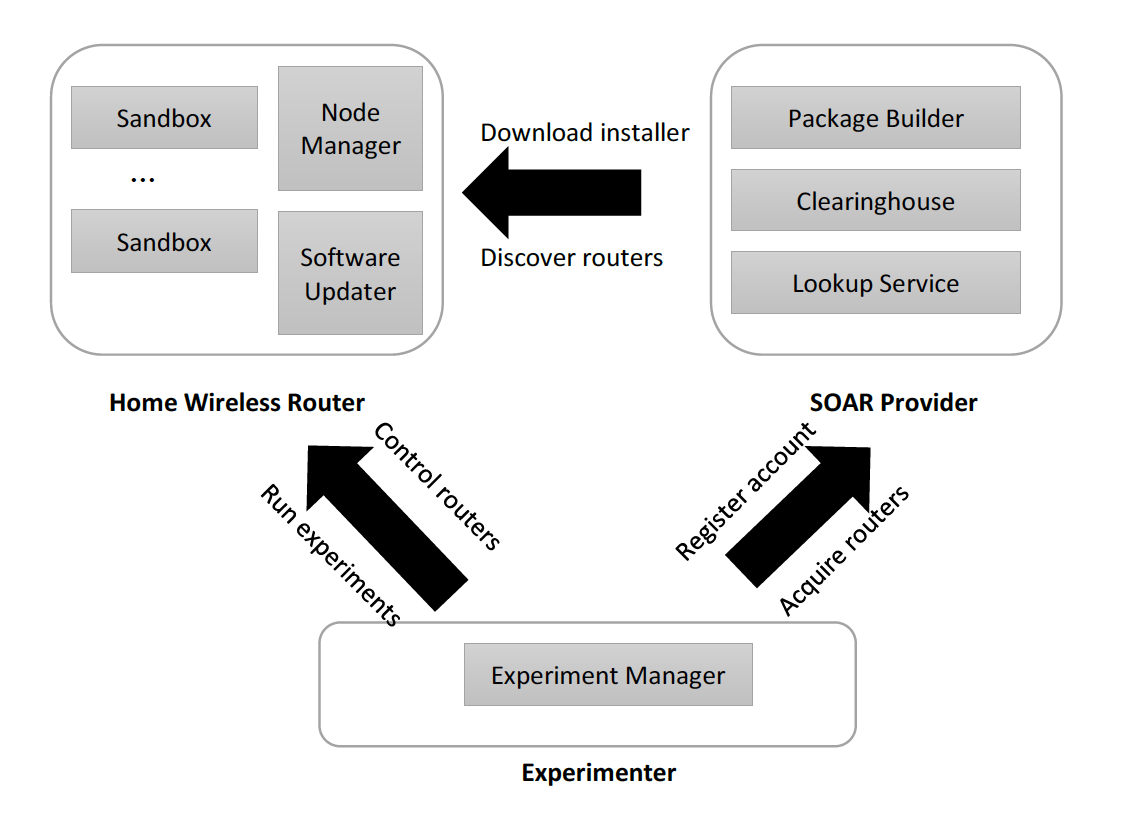
\includegraphics[width=0.8\columnwidth]{figure/soar-arch.png}
\caption{\sysname architecture and components.}
\label{fig-arch}
\end{figure}

\section{Platform Architecture}
The components in \sysname have three possible roles: the home wireless router (where an experiment runs), the platform provider (that distributes an installer with experimenter's credentials inside) and the experiment manager (where experiments are initiated).

\subsection{Home Wireless Router}
Home wireless routers provide computing resources for experimenters to use in their network measurements. To isolate experiment code from the router, the code is executed in a \textbf{sandbox} environment. The default sandbox in \sysname is \sandboxname, a subset of the Linux Kernel API constructed with the Restricted Python sandbox. When experimenters want to deploy their code on a remote router, they need a way to upload code into a sandbox and start it. The \textbf{node manager} listens for remote commands and mediates access to the sandboxes to ensure that only authorized experimenters can execute code in them. Finally, the \textbf{software updater} handles software updates. Once installed, automatically pushes any updates to the nodes instead of searching for new releases of the software manually.  

\subsection{Platform Provider}
The platform provider helps experimenters to pool and share platform resources. An experimenter can distribute a \sysname installer with his credentials inside and share it with router owners. To join \sysname, a router owner first acquires a \sysname installer. The sandbox, nodemanager, software updater and a set of public keys are packaged into this installer by a \textbf{package builder}. After an installation, the experimenter uses the public keys to register this router in a \textbf{lookup service} so that this router will be discovered by experimenters.

\subsection{Experiment Manager}
Experimenters use their local machines to initiate and control experiments on a router running \sysname. The \textbf{experiment manager} allows experimenters to deploy code into the sandbox and debug the result on a router running \sysname. The experiment manager first uses the looksup service to find the set of routers running \sysname that are associated with an experimenter. It then communicates with these routers, executing commands on the behalf of the experimenter.  

\section{API Design}
{\raggedright
\sysname is a network measurement platform designed to facilitate a broad range of experiments on a home gateway while controlling the impact on hosts' resources and network connectivity. A key challenge is selecting a programming interface that is both flexible (i.e., supports a rich set of network measurements) and safe (i.e., does not disrupt a normal user's Internet connectivity). Previous works on sandboxed, programming measurement environments, including the Seattle testbed suggested Repy could server as a useful environment for running network experiments. Considering our goal of supporting a wide range of network measurements on a home wireless router, we opt for extending a few capabilities of the Repy sandbox~\cite{cappos2010retaining}. The major goals of the sandbox are to provide security and performance isolation, and a portable programming interface across diverse device types. Currently this programming interface provides functions for networking, file system access, threading, locking, logging, and so on. These cover a broad range of network and file I/O capabilities. Repy is highly portable, and has been used in many network measurement projects, such as Content Distribution Network (CDN) Measurements~\cite{rafetseder2011exploring}, Video Streaming and Overlay Routing~\cite{eisl2011service}, Geographic Visualization of Mobile Network Data on open street map~\cite{open3gmap} and so on. Table~\ref{table:new_api} and \ref{table:Repy} provide a summary of our proposed API calls and the current set of measurement capabilities Repy supported. 

Network measurement platforms in today's home networks should support both active and passive measurement. Active measurements require injecting test packets into the network. Traditionally, active measurement tools, such as Ping~\cite{ping} and Traceroute~\cite{traceroute} were used to determine round-trip delays and network topologies. In comparison to the active measurement, the passive measurements do not inject test packets into the network. They need to capture packets and their corresponding timestamps transmitted by the platform. It can provide information such as availability, utilization, packet errors and discards~\cite{calyamactive}. We now briefly describe these capabilities corresponding to network measurements and detailed information about supported network measurements will be described in \S{\ref{sec.network_measurement}}.

\textbf{Basic Statistics.} \texttt{get\_network\_bytes}, \texttt{get\_network\_packets} and \texttt{get\_network\_interfaces} record aggregate network statistics for passively collected data. These methods read directly and parse data from \texttt{/proc/net/dev}. These are able to leverage the naturally-generated network traffic as passive measurements (particularly in the area of broadband characterization) by continuously monitoring the home gateway Internet connection.

\textbf{Wireless Information.} \texttt{scan}, \texttt{get\_station} and \texttt{wifi\_status} provide a python interface to low-level system calls. The function sanitizes the call arguments, parsing complex output and returning results to the caller. These methods use the \texttt{iw} command-line tool to trigger a new WiFi scan and to retrieve its results. \texttt{iw} is a new nl80211 based CLI configuration utility for wireless devices. It supports all new drivers that have been added to the kernel recently~\cite{iw}. They enable experimenters to study dense WiFi networks and home networks characteristics.

\textbf{Measurement Tool.} \texttt{ping} and \texttt{traceroute} serve as the basis for active measurements. These tools can be combined to build a wide range of measurement experiments. They also are able to contribute to local network debugging. Because these are commonly used, they are better to support on cross-platform experiments. In order to let these measurement tools perform on diverse operating systems, we use a pure raw socket method to implement it. 


\begin{table*}
\scriptsize
\centering
\begin{tabular}{|p{.2\textwidth}| p{.4\textwidth}| m{.6\textwidth}|}
\hline
\textbf{API}    &  \textbf{Description} \\
 \hline
 {\bf scan} & {\bf Collect the list of access points found with a WiFi scan. For each access point we collect BSSID, SSID, signal strength and channel number.} \\
\hline
 {\bf get\_station} & {\bf Record downlink statistics per associated client (e.g., Total packets sent, received, retried, client's signal strength in home wireless router).} \\
\hline
 {\bf wifi\_status} & {\bf Collect a list of WiFi channel information. (e.g., frequency, channel busy time, channel active time, channel receive time and channel transmit time).} \\
\hline
 {\bf get\_network\_interfaces} & {\bf Return a list of available network interfaces.} \\
\hline
 {\bf get\_network\_bytes} & {\bf Record information about the configured network interfaces. The statistics include metrics such total number of received or transmitted bytes, drops, errors.} \\
\hline
 {\bf get\_network\_packets} & {\bf Record information about the configured network interfaces. The statistics include metrics such total number of received or transmitted packets, drops, errors.} \\
\hline
 {\bf ping} & {\bf A pure python ping implementation using raw sockets.} \\
\hline
 {\bf traceroute} & {\bf Return the route packets take to network host. } \\
\hline
\end{tabular}
\caption {A summary of our proposed API calls.}
\label{table:new_api}
\end{table*}

\begin{table*}[]
\centering
\begin{tabular}{|l|l|lll}
\cline{1-2}
Network                                                                                                                                                                                                                                                                                         & File system                                                                                                                                         &  &  &  \\ \cline{1-2}
\begin{tabular}[c]{@{}l@{}}gethostbyname\\ getmyip\\ sendmessage\\ openconnection\\ socket.close\\ socket.send\\ socket.recv\\ listenforconnection\\ tcpserversocket.getconnection\\ tcpserversocket.close\\ listenformessage\\ udpserversocket.getmessage\\ udpserversocket.close\end{tabular} & \begin{tabular}[c]{@{}l@{}}openfile\\ close\\ readat\\ writeat\\ listfiles\\ removefile\end{tabular}                                                &  &  &  \\ \cline{1-2}
Threading                                                                                                                                                                                                                                                                                       & Miscellaneous                                                                                                                                       &  &  &  \\ \cline{1-2}
\begin{tabular}[c]{@{}l@{}}createlock\\ lock.acquire\\ lock.release\\ createthread\\ sleep\\ getthreadname\end{tabular}                                                                                                                                                                         & \begin{tabular}[c]{@{}l@{}}log\\ getruntime\\ randombytes\\ exitall\\ createvirtualnamespace\\ getresources\\ virtualnamespace.evalute\end{tabular} &  &  &  \\ \cline{1-2}
\end{tabular}
\caption{Repy key API functions to support issuing and programming measurement experiments.}
\label{table:Repy}
\end{table*}

\begin{table*} 
\scriptsize
\centering
\begin{tabular}{|p{.1\textwidth}| p{.3\textwidth}| m{.3\textwidth}|}
\hline
\textbf{Type} & \textbf{Parameters} & \textbf{Descriptions} \\
 \hline
 {\bf Passive} & {\bf Aggregate traffic statistics per associated client (e.g., Total packets sent, received, retried,
client\'s signal strength at AP)\newline nearby APs information \newline Channel utilization} & {\bf Home network usage patterns\newline Wireless network performance} \\
\hline
 {\bf Active} & {\bf Throughput, Latency, Loss, Jitter \newline traceroute \newline DNS lookups} & {\bf ISP performance \newline Large-scale topology mapping} \\
\hline
\end{tabular}
\caption {Measurement types supported by \sysname.}
\label{table:experiment}
\end{table*}

\section{Supported Network Measurements.}
\label{sec.network_measurement}
We begin by presenting examples of measurement efforts that benefit from the platform location (at the hub of a home networks) and supported capabilities. The list here is far from exhaustive; our design is general, and, hence, adaptable to a range of other experiments as well. Table~\ref{table:experiment} shows network measurements obtained from \sysname.

\begin{itemize}
\item \textbf{Wireless network performance:} Unlike prior wireless measurement studies that have deployed passive monitors~\cite{mahajan2006analyzing,raghavendra2009wi,papagiannaki2006experimental}, in our work, we collect wireless performance metrics using these home wireless routers as vantage points. Currently, \sysname supports gathering a variety of wireless network metrics, such as signal strength, tx/rx bitrate, SSID, BSSID, channel number, channel busy time. Unlike out-of-band wireless monitors, our wireless access points can exactly observe all traffic to and from its clients, correlate them with wireless performance, and hence conduct multiple types of measurements. In addition, a home router sits between the access link and wireless network so that it is better to identify and isolation problems between these two locations.

\item \textbf{ISP performance:} The home wireless router is ideally suited for measuring access link characteristics without being affected by confounding factors from the rest of the home network. A wide range of network I/O primitives we support can perform active measurement from home routers to a server, including speed test, performance diagnostics and so on. For example, it can download small binary files through a TCP connection from a web server to a router to estimate the connection speed.

\item \textbf{Large-scale topology mapping:} Many prior works from the research community have tried to understand the Internet's topology and connectivity by conducting \texttt{traceroute-like} measurements from multiple vantage points~\cite{paxson1996end,chen2009sidewalk}. A router-based platform that supports \texttt{traceroute} functionality would help researchers to extend their study.

\item \textbf{Home network usage patterns:} Since our platform sits between the access link and the rest of the home network, and acts as a continuous monitoring software, we can study home network usage patterns, such as the amount of traffic and the number of devices on the network at any given time. For instance, \texttt{get\_station} is able to gather information about the number of connected devices and \texttt{get\_network\_bytes} has the ability to know the amount of network traffic.    
\end{itemize} 
\par}
\section{Security}
\label{sec.security}
With the rapid development of smart home technology, it becomes essential to focus on home network security and privacy. Since \sysname deploys on the home wireless router, any bugs can have a significant impact on a home network. For instance, attackers may obtain the control of the home networks through a malicious attack. 

To understand how to prevent attacks, we first considered the different kinds of attacks. We observe that they fall into three types: (i) Denial of service attack (e.g., Packet flooding, SYN flooding~\cite{eddy2011syn}): overwhelm targets with a flood of network traffic to drain end host resources or control/drain resources on routers, (ii) Injection attack (e.g., Remote exploits~\cite{shellcode},  spoofing attack~\cite{bishop1996attack}): create a few ``magic'' packets to implement spoof attack or exploit attack. (iii) Insider attack (e.g., Network eavesdropping): malicious insiders intentionally eavesdrop, steal, or damage information to violate user's privacy.

To prevent these three types of attacks, \sysname uses a sandboxed environment named Repy for security isolation and performance isolation.
 
\begin{itemize} 
\item \textbf{Security isolation:} The sandbox must be able to ensure the execution safety of experiment code while representing as little risk to the host as possible. The Repy sandbox in \sysname uses language-based isolation and is implemented in Python. In addition, Repy uses a security layer to push library functionality out of the sandbox kernel, thereby helping to mitigate the impact of bugs in libraries~\cite{cappos2010retaining}. As a result, an experimenter can enforce a policy upon a Repy sandbox without needing to change the TCB (trusted computing base).  
\item \textbf{Performance isolation:} Resource consumption is the biggest issue for a distributed system. In the home network, we need to share our platform with an unidentified home wireless router. If vulnerabilities come into effect\cite{joshi2013survey}, the rate of resource consumption may degrade the performance itself, and the performance of other applications in real networks~\cite{joshi2013survey}. Therefore, \sysname must control the load its experiments impose on the routers, as well as minimize the impact of real user's network connectivity. To achieve this, \sysname should limit consumption of host's resources, include the amount of CPU and memory used, network and disk I/O. To control CPU and memory utilization, \sysname monitors the amount of CPU and memory available to a experiment. To control network and disk I/O, \sysname checks calls that access these resources and prevents their execution if they exceed a predefined limits. 
\end{itemize}

Through performance isolation, the volume of an experiment's network traffic and the available resources for experiments is restricted based on the quota the router owner predefines. Therefore, denial of service attacks are impossible because our platform does not allow to launch a sustained flood of traffic to other hosts. In addition, since the sandbox controls CPU, memory, bandwidth, disk I/O and other resources, \sysname is able to control the load of its experiments imposed on a wireless router. Through security isolation, experimenter has the ability of setting up policies for library and returned data. For instance, if one wants to restrict access to a specified functionality's parameter or returned value, this can be added in a secure policy without changing Repy. To mitigate the second and third types of attacks, we could block a few functionalities that may pose risks to home networks, and anonymize sensitive information that might leverage users' privacy. Detailed information is discussed in \S{\ref{sec.privacy}}. 

\section{Privacy}
\label{sec.privacy}
Although a rich set of capabilities enhance the convenience of user interfaces and application usefulness, they also raise serious privacy concerns. For example, network traffic volume over an interface and the information from connected devices in home networks produce a rich history that can lead to behavior prediction, which can invade user privacy. 

In order not to allow measurements to exfiltrate sensitive information from a home gateway, \sysname provides a framework of reference monitors~\cite{ref}, to enforce mandatory access control to sensitive data in real time. Figure~\ref{fig-reference} shows an overview of the reference monitor. Instead of modifying the sandbox, \sysname allows users to decide not only what information experimenters can capture on their routers, but also how much information they can share with others. \sysname allows router owner to add the privacy filters they wish to apply. These may range from sharing some home network device information with an experimenter by just blocking MAC addresses, to completely denying access to network traffic statistics. For a particular experiment, a privacy policy might based on the type of network measurement, and the capabilities can be passed through, filtered, or dropped by the reference monitor. For an experimenter who wants to learn about Internet censorship, a filter might perform an action such as removing access point information from WiFi scans and network traffic volume information in home networks, only allowing access to ping and traceroute functionality. These privacy filters are easily built and disseminated to router owners. Therefore, \sysname is able to handle the second and third types of attacks in \S{\ref{sec.security}}. 

\begin{figure}%[h]
\centering
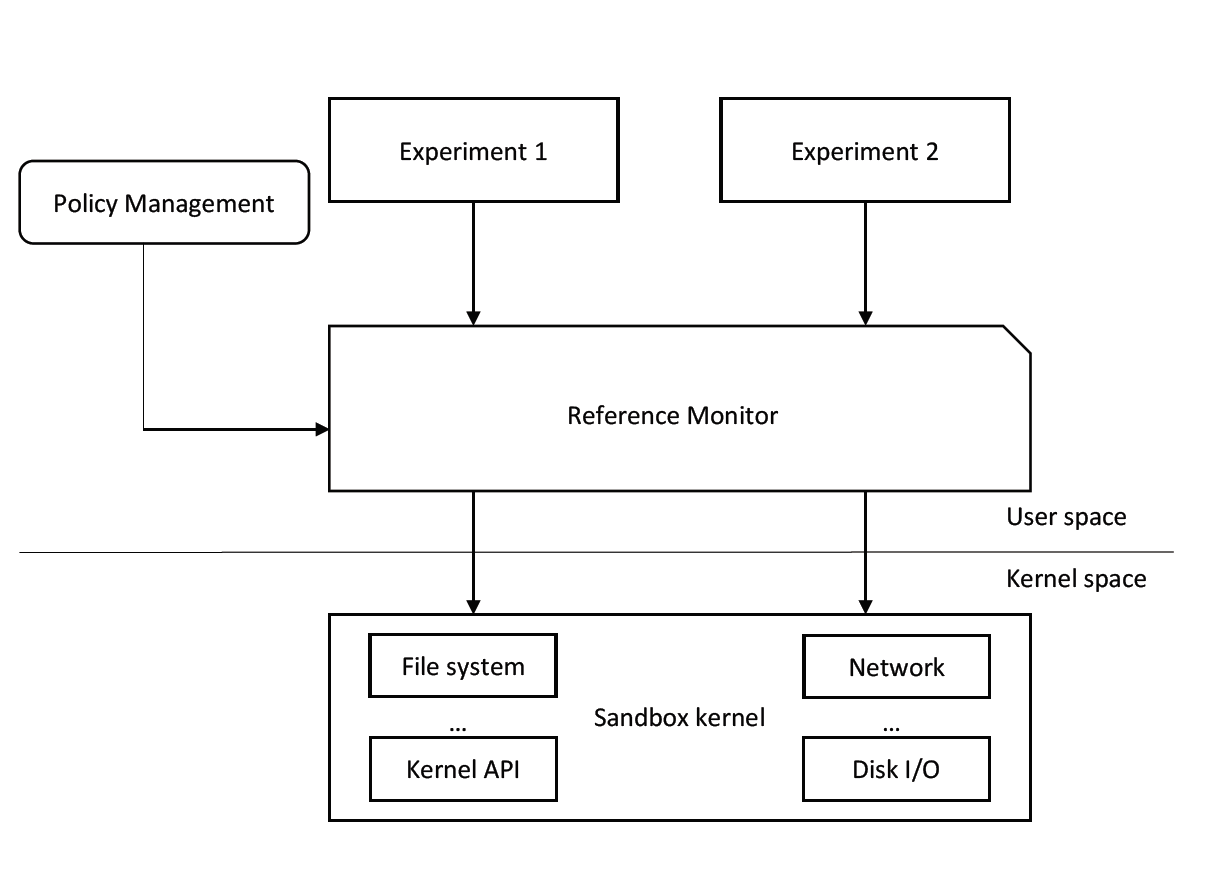
\includegraphics[width=0.8\columnwidth]{figure/referencemonitor.png}
\caption{Overview of reference monitor. The original Repy interface and the added API together provide the OS level sandbox kernel on a home wireless router. Before an experiment can access data, different policies can be combined together as a set of filters to protect users' privacy.}
\label{fig-reference}
\end{figure}


\chapter{Implementation} 
\label{sec.implementation}

Based on the design introduced in \S{\ref{sec.design}}, we implement a 
secure network testbed. We describe the implementation details of our system 
in this section. It is important to acknowledge that the \sysname benefits from the design and implementation of Seattle Testbed, an open experimental platform for researchers and educators to understand the real world network. Over the past six years, the Seattle Testbed has been used in a variety of different experiments and its use is spread across the world. A core design principle of this testbed is the implementation of Repy sandbox on user devices. The sandbox has several goals. First of all, it must be able to run experiment code while representing as little risk to user's security as possible. For instance, programs are only allowed to operate inside of a sandbox, ensuring user's sensitive information on host are kept safe and private. In addition, sandbox must provide performance isolation for experiment code to prevent them from consuming too much CPU, memory, disk I/O and network bandwidth. The basic design of the Repy for OpenWrt described below was leveraged from the Seattle design.

\section{Core components}
\subsection{Sandbox}
\label{sec.sandbox}
The core sandbox of \sandboxname, which is extended from Repy (Restricted Python), a Python-based programming language sandbox that minimizes the risk of bugs by providing security isolation and performance isolation. Experimenters in \sysname use this Python-like programming interface to write experiment code. Currently. Repy provides programmers with the ability to read and write files on the disk, send TCP and UDP traffic and some utility methods to retrieve time etc. In order to run broadband and wireless network experimentation on home wireless routers, \sysname extends the Repy and adds the capabilities to access linux kernel API and active measurement tools (e.g., Ping, Traceroute). The programming interface exposed to the repy-scripts has been extended to include methods to list available access points and connected clients, receive network traffic data from \textit{\\proc} file system and do common active measurements (Ping and Traceroute). To avoid resource limitation, we define a non-renewable and fungible resource\cite{li2015fence} (\textit{procfs}) to control the resource of reading \textit{\\proc} file system. 

Another important feature of \sandboxname allows us to define a policy for its programming interface. For example, the sandbox can anonymize the MAC address of available access points and blacklist home user's LAN. The policy enforcement is presented in \S{\ref{sec.policy}}. We focus on the security and performance isolation of \sandboxname in this section.
\begin{itemize}
\item \textbf{Performance isolation: }Each router running \sysname uses an uniform resource control method to allocate a fixed percentage (usually 50\%) of the router's CPU, memory, brandwidth, disk and other resources to one or more sandboxes. To achieve this, Repy uses operating system hooks to monitor the amount of CPU and memory available to an experiment. To restrict other resources such as network bandwidth and disk I/O, Repy checks those calls that access these resources, and preventing or delaying the execution of these calls if they exceed configured quota. When sandbox is started, it reads a configure file that lists the resources allocated to the experiment. Each line contains a resource type and quantity. For example, \textit{resource diskused 100000000} means that 100 million bytes disk memory can be used at most. Due to this isolation, sandbox does not allow experiment to consume a lot of resources and ensure experiment not affect Internet connectivity.

\item \textbf{Security isolation: }Repy sandbox has a small, self-contained kernel as its trusted computing base (TCB). In order to minimize the risk of bugs, the TCB is small (only include classic Python classes) so that it is less likely to have security risks than other complex kernels. This sandbox also uses \textit{security layers} to push library functionality out of the sandbox kernel, therefore it is helpful to mitigate security risks in libraries. 

\end{itemize}
\subsection{Package Builder}
\label{sec.packagebuilder}
Any experimenter can easily obtain a customized installer for \sysname which provides access to sandboxes in any way. The goal of package builder is make it incredibly easy to post our platform to OpenWrt. Currently we use OpenWrt SDK to build installer. These can be given out by an experimenter who does not want use a clearinghouse. In addition, these installers can be bundled with other components to allow the experimenter direct control over safe experimental sandboxes on their end user devices.

\subsection{Node Manager}
\label{sec.nodemanager}
Node manager\cite{nodemanager} ensures that sandboxes are correctly assigned to experimenters and experimenters can control those sandboxes safely. The Node manager is based on prior work on Seattle Testbed, but is customized to the OpenWrt. For example, \sysname runs on a home wireless router as background process. Starting it at booting time of the router is implemented by an init.d script instead of crontab. Cryptographically signed messages is used to perform authentication of remote experimenters who are identified by their public keys. An experimenter can perform actions on the sandbox such as starting and stoping an experiment, uploading code, collecting files and data. The node manager is running in a sandbox to check whether the interface is accessed. The node manager also includes code to traverse NAT gateways and firewalls so that it is contactable even if the router does not have a public IP address. 

\subsection{Software updater}
\label{sec.softwareupdater}
Software updater allows SOAR-enabled router to search for and update new release automatically. It runs in background, sleeps some random amount of time (30min - 1hour) to check with the package builder if there exists a new update. It then downloads the new installer from package builder and replaces the old installer. 

\subsection{Lookup service}
\label{sec.lookupservice}
A lookup service allows experimenter to locate the corresponding sandboxes. We currently use OpenDHT\cite{rhea2005opendht} as a distributed way to store data. Each sandbox advertise their availability via OpenDHT using a public key. OpenDHT runs on a variety of PlanetLab nodes and replicates data.

\subsection{Experiment manager}
\label{sec.seash}
An experiment manager provides experimenters with a simple interface for interacting with the resource manager on remote devices. The primary interactive service manager used in \sysname is \textit{seash}\cite{seash}. It provides an interactive shell to the experimenters. \textit{seash} exchanges cryptographically signed communication with sandboxes to control experiments and upload files. Also, the experiment manager supports contacting routers which in networks behind NAT gateways and firewalls to satisfy the reality of today's network.

\section{Sandbox extensions}
\label{sec.extensions}
Extensions enhance the functionality of the Repy sandbox and allow a wide range of network measurements on home wireless router. First, we implemented system hooks call \textit{openwrt module} to interact with a variety of wired and wireless network information through Linux kernel API. Currently, implemented \textit{openwrt module} is supported to learn about configured network interfaces statistics, connected devices, nearby WiFi access points and channel utilization. While \textit{openwrt module} is the system hooks with read access to valuable data, they can not modify data. Additionally, we also implemented a \textit{general modules} to provide two active measurement tools (Ping and Traceroute). We choose a pure raw socket method to implement them so that they will be supported across a variety of operating systems. 

\textbf{Protecting command injection.} Command injection is an attack which execute arbitrary commands on the host operating system by a vulnerable application. The possible reason of command injection attacks is insufficient input validation. \sysname sanitizes the call arguments, handles onerous output parsing, and returns results to the caller. One example is \textit{scan} implementation. This function will run a system command \textit{iw dev interface\_name station dump}. We will check whether interface name is legal, any illegal arguments will pose a security risk, such as \textit{;ls} is able to show files in current directory. \sysname API never allows invocation of arbitrary system calls.

\begin{figure}%[h]
\centering
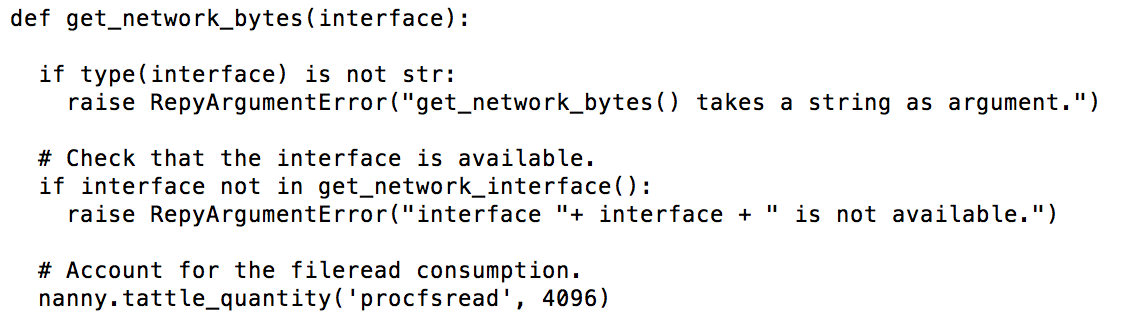
\includegraphics[width=0.8\columnwidth]{figure/nanny.png}
\caption{Here is an example of resource control in \sysname sandbox}
\label{fig-nanny}
\end{figure}

\textbf{Resource control.} Resource control is an important security mechanism. It provides protection from accidental or deliberate over-usage of resources by APIs affecting the service level of end host. Each new functions in SOAR-Repy define a resource type to record the amount of resource they consume. The specific function made depends on the type of resource being consumed. Figure \ref{fig-nanny} shows some of codes in \textit{get\_network\_bytes()}. First of all, we check whether the argument is legal and available. The \textit{tattle\_quantity()} call charges for the consumed fileread. When a \sysname starts, it reads a text file that lists the resources allocated to the platform. Each line contains a resource type and quantity. For example, \textit{resource procfsread 100000} sets the allowed consumption of reading \text{\\proc} filesystem to 100 thousand bytes. When experiment codes try to exceed the limit, it will be forcefully killed.

\section{Sandbox policies}
\label{sec.policy}
In order for router owner to participate safely in \sysname, he should have the ability to decide policies on his own. For instance, he should know the amount of resources \sysname will use on his router and the capabilities experiment code can access to. We have mentioned the resource control in \S{\ref{sec.sandbox}}. To restrict capabilities, the sandbox in \sysname provides a flexible policy enforcement method that uses Repy's security layer to help router owner to decide policies. Sandbox can interject code to control the behaviour of these calls through a system call interposition technique. Using this technology, a sandbox policy can (1) restrict capability access, such as blocking sending TCP or UDP packet to protect LAN, and (2) reduce precision of returned data from a router, such as returning the number of connected devices rather than detailed information of each connected device.

\subsection{Reducing Data Precision}
Our sandbox may provides potentially inappropriate functions such as network traffic capture that disclose the home network behaviour pattern of router owner. This kind of policies are able to change the behaviour of a function such as it can disable the returned value and the precision of a specified value returned. For instance, security layer could truncate access point MAC address to the manufacturer ID.

\begin{figure}%[h]
\centering
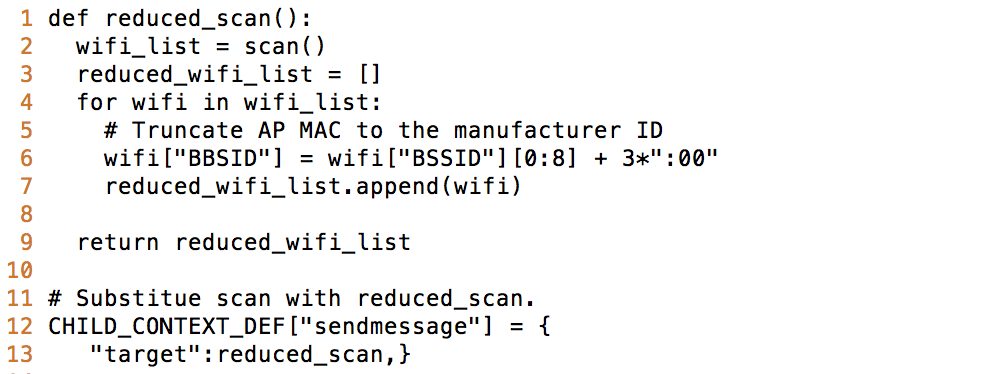
\includegraphics[width=0.8\columnwidth]{figure/example.png}
\caption{An example code of security layer}
\label{fig-examplecode}
\end{figure}

As shown in figure~\ref{fig-examplecode}, whenever experiment code calls \textit{scan()}, the security layer above replaces it with \textit{reduced\_scan()}. Therefore, security layer is able to ensure router owner's policy.

\subsection{Restricting Capability Access}
This kind of policy is able to allow experimenters to restrict the code on home wireless router. For example, the experimenter may wants to restrict part of functionalities to satisfy router owner's need. It is also useful to save time to vet experiment code because most harmful capabilities are restricted. As a result, \sysname is able to maintain containment of experiment code despite bugs in libraries.
 
\chapter{DEPLOYMENT EXPERIENCE} 
\label{ssec.deployment}
Deploying \sysname in a real-world environment is essential to the study and evaluation of home network's availability, performance and reliability. We want our platform to observe real user traffic from any Wi-Fi connected devices in a home; at the same time, we want to maintain the flexibility to deploy experiment code quickly and easily, without any impact on users experience. To achieve this goal, we integrate \sysname with a production network.

We deploy our platform on a TP-Link TL-WDR3600 router, which has a 560 MHz MIPS processor, 8MB of flash storage, 128MB of RAM and a dual-band wireless interface. We replace the router's default software with a custom version of OpenWrt Chaos Calmer~\cite{openwrt}. The 802.11 interface operates at both 2.4 GHz and 5 GHz bands. The location is in an office building on the NYU campus. This hardware is limited, even when compared to other embedded mobile devices like smartphones, yet it is powerful enough to reliably support a variety of measurement experiments.

To simply port to the OpenWrt environment, we build custom package management utilities on the top of \texttt{ipkg} because \texttt{ipkg} package manager is able to resolve dependencies with packages in the repositories. If this fails, it would report an error, and terminate the installation of that package. To let our platform start at boot time automatically, we opt for init.d script instead of crontab because \texttt{@reboot} is an extension to the BSD cron.d, not supported by Busybox cron.d.
\chapter{EVALUATION} 
\label{sec.evaluation}
In this section, we demonstrate SOAR's utility by implementing three example use cases that together ``play'' different types of its API: comparing the performance of 2.4 GHz and 5 GHz bands, studying channel survey statistics and home wireless environment. Our goal is to illustrate how \sysname can support a variety of measurement needs.
\section{Method}
\subsection{Measurements}
\label{ssec.measurements}

We perform both active and passive measurements of network traffic from home wireless access point and correlate those measurements with the wireless metrics for the corresponding traffic. Passive measurements reflect the actual performance more accurately. Unlike passive measurement, active measurements generate additional network traffic that are sent over the network to, for example, measuring the time it takes for the packet to reach the other end of the network (TCP RTT) and the available capacity of a wireless network. However, active measurements might introduce contention or disturb the normal traffic flow. Combining active and passive measurements is called hybrid measurements. 

To generate the maximum possible send/receive rate that \sysname can achieve. we use \texttt{socket.send}/\texttt{socket.recv} within a tight loop and using a timer to saturate the available network bandwidth. We perform all tests between clients on the same wireless network and the home access point. We collect network traffic statistics and channel survey information from both wireless interfaces on the access point. The data collection on the access point is done by periodically querying some data exposed by our platform's supported API (e.g, \texttt{get\_network\_bytes} and \texttt{wifi\_status}). Our sandbox environment ensure that monitoring should not have any negative impact on the routers. 
 
\subsection{Deployment Experience}
\label{ssec.deployment}

We deploy our platform on a TP-Link TL-WDR3600 router, which has a 560 MHz MIPS processor, 8MB of flash storage, 128MB of RAM and a dual-band wireless interface. We replace the router's default software with a custom version of OpenWrt Chaos Calmer~\cite{openwrt}. The 802.11 interface operates at both 2.4 GHz and 5 GHz bands. The location is in NYU campus, which is an office building. 

\subsection{Metrics}
\label{ssec.metrics}

Our metrics are based on supported APIs provided by \sysname. We use channel busy time as an indicator of the channel utilization, and with channel transmit time and receive time to calculate the external interference. We also report the achieved throughput generated by the running experiments. We next elaborate on our metrics.

\textbf{Channel busy time:} The channel busy time is the amount of time the primary channel was sensed busy. This seems to be about the same as the sum of channel transmit and receive times, unless there is a lot of external interference (like another busy Wi-Fi network on the same channel)\cite{channelsurvey}. We report the channel busy time every 30 seconds. Typically, a lower channel busy time is an indicator of good throughput and negligible interference.

\textbf{Channel transmit and receive time:} The channel transmit and receive time are the amount of time the radio spent transmitting and receiving data. In general, the following relation seems to be like that: 

\(\frac{t_{channel-tx} + t_{channel-rx}}{t_{channel}} < \frac{t_{channel-busy}}{t_{channel}} < 100\%\).

\textbf{Achieved throughput:} Our platform periodically (30 seconds) reports the actual throughput for each interfaces. Achieved throughput is the actual total number of bytes over time, and it captures the actual demand on the wireless network. This metric depends on the experiment's data rate and is bounded by the wireless effective throughput. The throughput is computed as the transmitted bytes over one second period.

\textbf{TCP round-trip time (RTT):} RTT is the difference between the time of the data and TCP SYN packets and its corresponding acknowledgements. As this RTT increases, it can have an adverse impact on performance, especially for applications that are latency sensitive. Measuring the RTT between the access point and the home devices is important for us to understand wireless performance.

\textbf{Additional metrics:} Our platform reports each station's \texttt{tx} retries and \texttt{tx} failed. \texttt{tx} retries and \texttt{tx} failed are reported only in downlink (gateway to station) and we use them as an additional performance indicator. Finally, our platform also reports unix timestamp along with other metrics. This is used to help me calculate throughput and study network usage pattern. 

\section{Usecase: Comparing the wireless performance of 2.4 GHz and 5 GHz bands}
\label{sec.usecase1}

Better use of 5 GHz to improve wireless performance on a dense WiFi network is a common strategy because there are generally fewer devices in the 5 GHz band (This means that the noise floor is much lower) and 5 GHz band has less non-WiFi interference. Thus our hypothesis was that devices on the 5 GHz band would perform better.

We use \sysname to evaluate the wireless performance of network traffic on 2.4 GHz and 5 GHz band. Our focus is not on improving performance, but rather to underscore how we can use \sysname to gain useful insights into a real network.

For this experiment, the router that we use enables both 2.4 GHz and 5 GHz radios, which allows us to compare the performance of these two bands. To ensure there are similar network traffic on 2.4 GHz and 5 GHz band, we performed a multi-threaded TCP experiment on \sysname to send intermittent TCP packets to clients which connected 2.4 GHz and 5 GHz band, respectively. Then we collect network traffic statistics to compare wireless network performance.

\begin{figure}
\begin{subfigure}{0.5\textwidth}
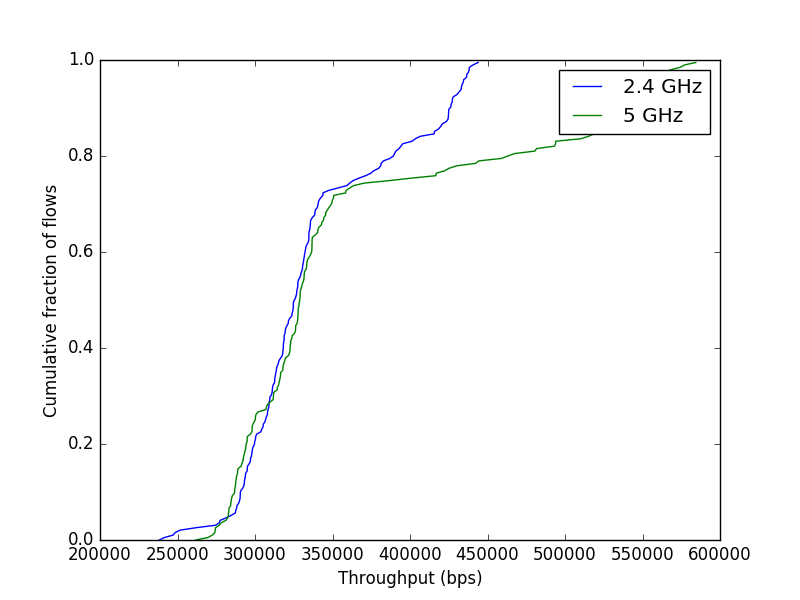
\includegraphics[width=\linewidth]{figure/throughput(5g_vs_2g).png}
\caption{Network traffic in the 5 GHz band achieve higher throughput} 
\label{fig:throughput}
\end{subfigure}
\hspace*{\fill} % separation between the subfigures
\begin{subfigure}{0.5\textwidth}
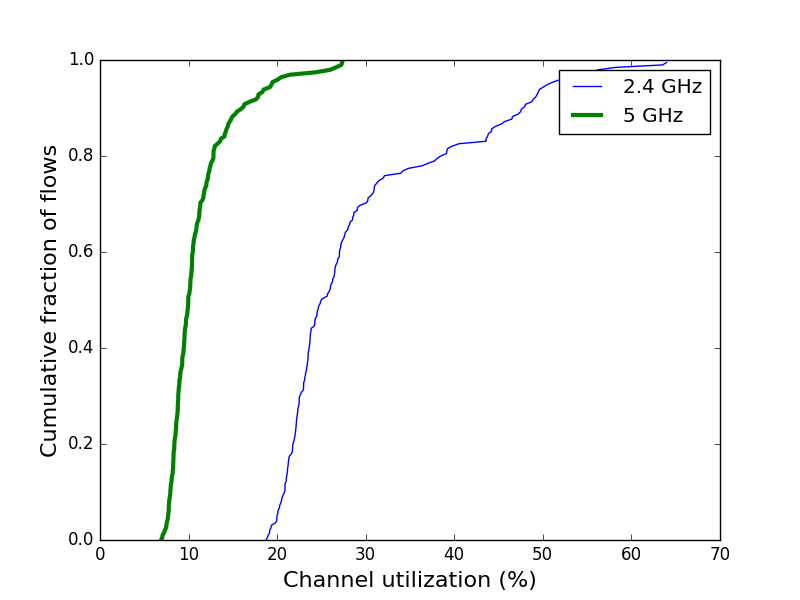
\includegraphics[width=\linewidth]{figure/channel_utilization(2g_vs_5g).png}
\caption{Network traffic in the 2.4 GHz band experience higher channel utilization.} 
\label{fig:utilization}
\end{subfigure}
\hspace*{\fill} % separation between the subfigures
\begin{subfigure}{0.45\textwidth}
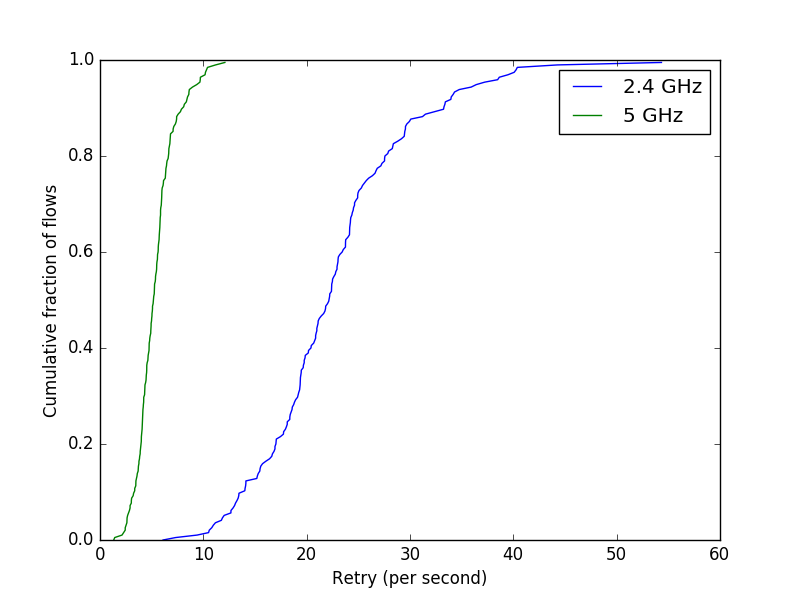
\includegraphics[width=\linewidth]{figure/retries(2g_vs_5g).png}
\caption{Network traffic in the 2.4 GHz band experience higher tx retries.} 
\label{fig:retries}
\end{subfigure}
\hspace*{\fill} % separation between the subfigures
\begin{subfigure}{0.5\textwidth}
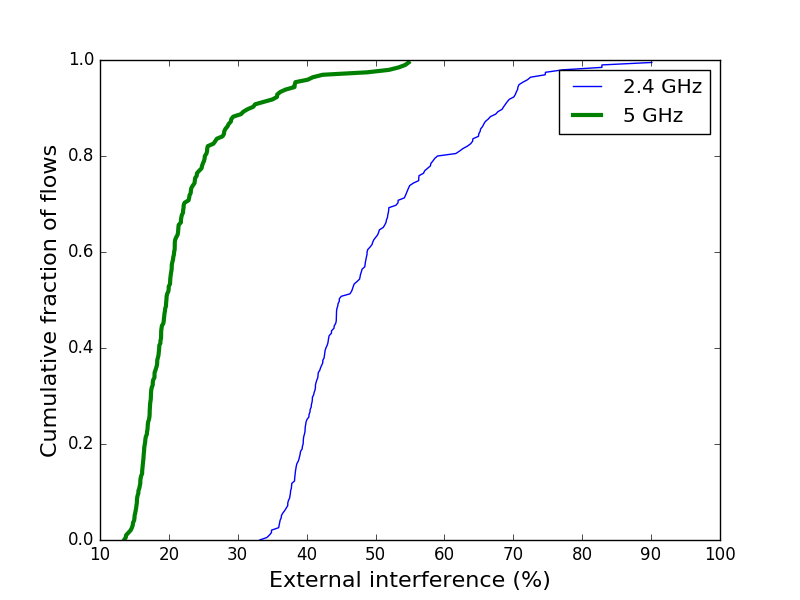
\includegraphics[width=\linewidth]{figure/external_interference(2g_vs_5g).png}
\caption{Network traffic in the 5 GHz band has less external interference.} 
\label{fig:interference}
\end{subfigure}
\caption{Characteristics of flows in the 5 GHz vs. the 2.4 GHz spectrum.} 
\label{fig:5gvs2g}
\end{figure}

\textbf{2.4 GHz vs. 5 GHz:} We use throughput, channel utilization, retransmission times and external interference as our indicator of wireless performance because we can obtain these metrics easily from our supported APIs. We calculate throughput as follows: using \texttt{get\_network\_bytes} to provide TCP statistics. We study the aggregate TCP throughput achieved during the captured lifetime of the network traffic. We compute the average throughput at every one-second interval by the divisor of aggregate TCP throughput and the difference between the correspond timestamp. \texttt{get\_station} can help us obtain the number of retry packets at each clients. We also compute channel utilization and external interference as the percentage of channel busy time and external interference time in any given one-second interval. 

We see that the use of 5 GHz improves performance, reducing channel utilization, external interference and retransmission rate. Figure \ref{fig:throughput} shows the network traffic in the 5 GHz band achieve higher throughput. Figure \ref{fig:utilization} shows the channel utilization in 2.4 GHz are much higher than 5 GHz. Figure \ref{fig:retries} shows the retransmission times per 40 seconds; the result shows that transmissions are more common in the 2.4 GHz band. Figure \ref{fig:interference} plots the CDF of the external interference for all network traffic for both the 2.4 GHz band and the 5 GHz bands. The 5 GHz band has less interference as signal does not propagate well through walls. A limiting factor to identify the real wireless performance is the lack of contention and feedback from external sources (i.e., local contention and non-WiFi wireless devices). However, we still leverage channel busy time to detect airtime utilization.

\begin{figure}
\centering
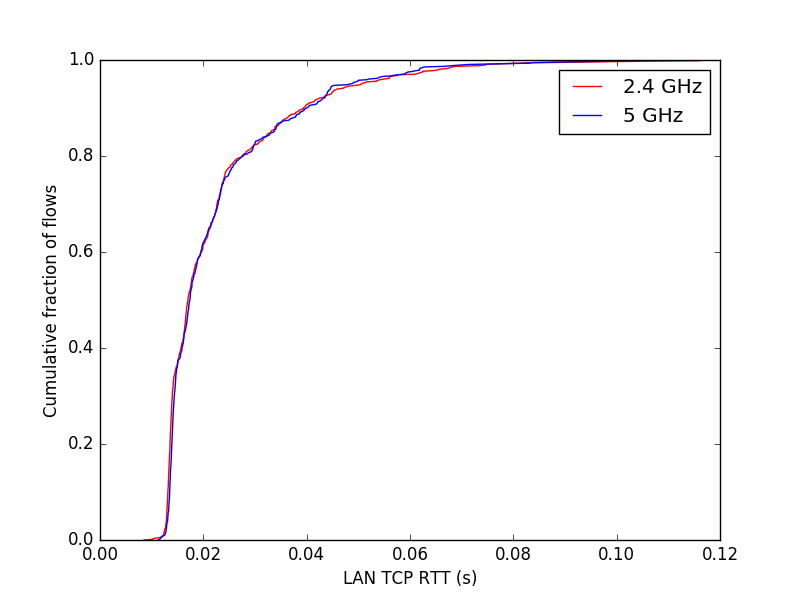
\includegraphics[width=0.5\textwidth]{figure/tcp_rtt.png}
\caption{LAN TCP round-trip time for different bands (e.g,. 2 GHz, 5 GHz).} 
\label{fig:tcprtt}
\end{figure}

\textbf{TCP round-trip time is similar on 2.4 GHz and 5 GHz band.} We calculate TCP round-trip time as follows: using the home router as vantage point and calculate the time between a TCP packet coming and its respective TCP acknowledgement from a connected client. We collected the TCP round-trip between the wireless home router and a wireless client on 2.4 GHz and 5 GHz band. Figure \ref{fig:tcprtt} plots the CDF of the TCP round-trip times for all network traffic for both the 2.4 GHz band and the 5 GHz band. Interestingly, the result shows that TCP round-trip time on 2.4 GHz and 5 GHz band are similar. To better understand our finding, we compute packet loss rate, which is measured as a percentage of packets lost with respect to packets sent. Packet loss rate on 2.4 GHz and 5 GHz band is 67.9\% and 75.7\%, respectively. This might be a factor to explain why there are different throughputs on each bands.  

\begin{figure}
\centering
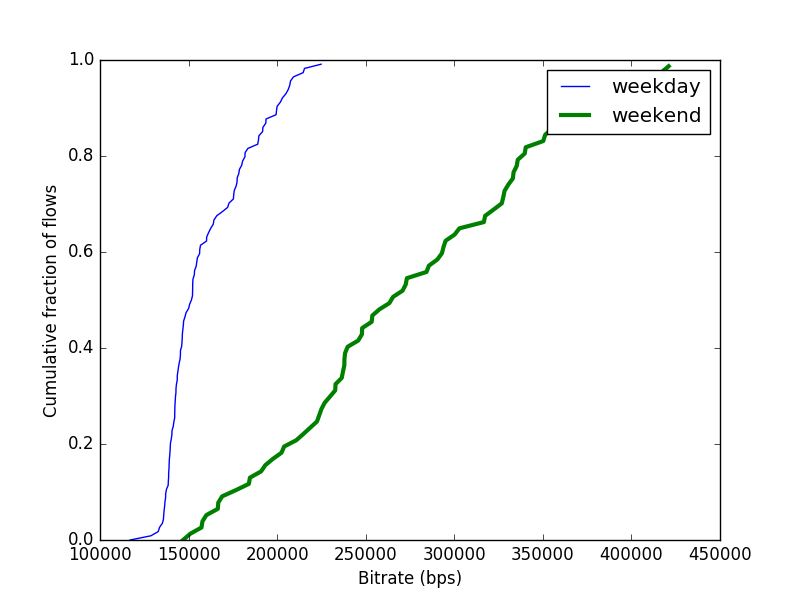
\includegraphics[width=0.5\textwidth]{figure/bitrate(weekday_vs_weekend).png}
\caption{Bitrate on weekday and weekend in an office building in NYU Brooklyn campus. Weekend bitrate is more than weekday bitrate.} 
\label{fig:compare}
\end{figure}  

\section{Usecase: Studying channel survey statistics}
\label{sec.usecase2}

\begin{figure}
\centering
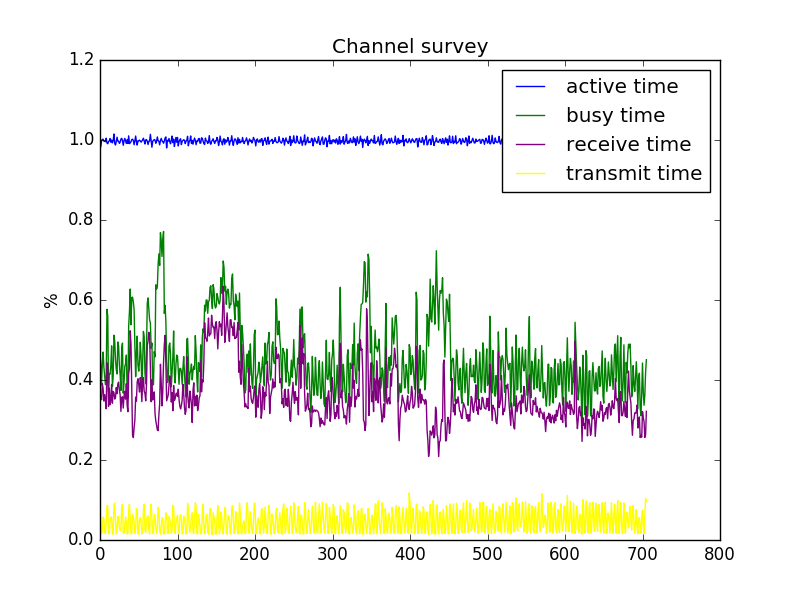
\includegraphics[width=0.5\textwidth]{figure/channel.png}
\caption{Channel survey metrics in 2.4 GHz band through \texttt{wifi\_status}.} 
\label{fig:channelsurvey}
\end{figure}

Measurement studies show that congestion in a wireless network leads to lower overall network throughput and capability. The lack of techniques to identify and characterize congestion in wireless networks has prevented relevant research. To better understand congestion in wireless networks, \sysname provides the capabilities to explore radio channel channel utilization data. 

As \cite{channelsurvey} did before, we replicated this experiment through our \sysname platform. We use \texttt{wifi\_status} to collect channel busy time, active time, transmit time and receive time. Figure \ref{fig:channelsurvey} shows the channel survey statistics captured in 2.4 GHz band. We find that channel active time is the same as running time if you don't change channels. Channel busy time seems to be the same as the sum of transmit time and receive time, unless there is a lot of external interference (e.g, heavy external traffic on the same channel, non-WiFi devices).

Next, we study the potential indicator can cause the degradation of a wireless performance. We therefore investigate this, by correlating the throughput (which can be caused by interference) with the airtime utilization and external interference. Interestingly, we find that there is no strong correlation between wireless performance and airtime utilization or external interference. Table \ref{table: Correlation} shows the correlation between these indicators available at the AP and the observed TCP throughput from our continuous measurements. We observe that, lower airtime utilization does not necessarily result in higher TCP throughput. Note that we need to interpret our findings with cautiousness. First, the TCP traffic do not saturate the wireless link. This is because our platform is deployed on resource-constrained devices. Therefore, we do not have fine-grained feedback of highest airtime utilization or external interference. Second, our platform does not capture all the activities in the home wireless network, which would allow us to gain deeper insights for the correlation between throughput and airtime utilization. Third, our platform does not report the traffic from nearby networks, which would allow us to gain deeper insights from the external interference.

\begin{table*}[]
\centering
\begin{tabular}{ |c|c| }
\hline
Indicator               & Correlation Coefficient  \\ 
\hline
Airtime               & -0.094  \\ 
\hline
External Interference & -0.031 \\ 
\hline
\end{tabular}
\caption{Correlation of metrics with the observed TCP throughput.}
\label{table: Correlation}
\end{table*}

\section{Usecase: Studying home wireless environment}
\label{sec.usecase3}

\textbf{Within a home network, individual devices experience different wireless performance at different time.} Figure \ref{fig:compare} uses the WiFi data set to show throughput of wireless network during each hour of day, partitioned into weekday and weekend. We observe a diurnal throughput in home network in a office building at various times of day on a weekday and weekend. We see that throughput is higher at weekend than weekday, which may result from there are less external interference (e.g., surrounding access points, clients).

\textbf{Home WiFi neighbourhood.} We next leverage the feedback from our platform to analyse its WiFi neighbourhoods. Overall, we observe the number of neighbouring SSIDs around our wireless router which is located in an office building. The number of neighbouring SSIDs varies between 26 and 64. The average number is around 46.45. We also observe network density in the night (between 0:00 am and 6:00 am), the average number is around 48.83. Therefore, the network density does not vary a lot in the day and night (possibly employees work late or there is no automation to manage these wireless routers).

\begin{figure}
\centering
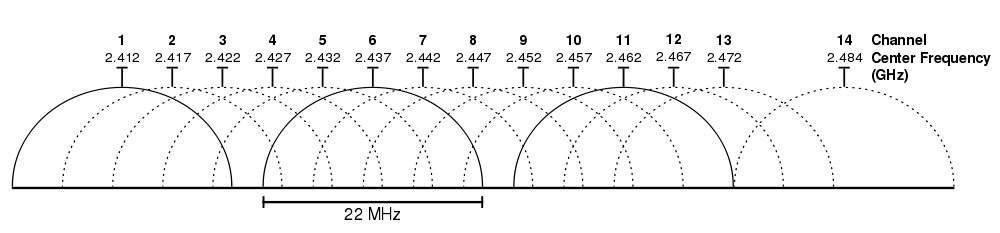
\includegraphics[width=0.8\textwidth]{figure/2GHz_WiFi_channels.png}
\caption{There are three channels that do not overlap in the on 2.4 GHz : 1, 6 and 11.} 
\label{fig:channels}
\end{figure}

In the 2.4 GHz band, 1, 6 and 11 are the only non-overlapping channels. Selecting one or more of these channels is an important part of setting up your network correctly. As we can see from Figure \ref{fig:channels}, co-channel interference is where devices take turns talking, so the more devices on one channel, the longer it takes for a device to talk since it has to wait for its turn. In our dataset we find that access points in this building mostly use channel 1, 6, and 11. Specifically, 42\% of access points use channel 6, 21\% of access points use channel 1, 28\% of access points use channel 11 and the rest use other overlapping channels. In general, we expect there are equal network traffic in channel 1, 6, 11, respectively. However,  many wireless routers automatically select the channel for you upon initial setup, it could lead to slow Wi-Fi speeds and interference. 

Overall, our results show that majority of APs (91\%) observed in an office building in NYU campus select non-overlapping channels. However, most of them are distributed on channel 6 indicating that they might use static channel configurations and rarely get configured once they get deployed. Our study also found a behavioural pattern: most companies in the office building do not turn off routers after work time.   
\chapter{CONCLUSION}
\label{sec.conclusion}
In this thesis, we presented \sysname, an experimental platform for home Wi-Fi routers. \sysname provides a programmable interface for writing and launching measurements without compromising user's privacy and minimizing the impact on the performance of home wireless routers. The greatly reduced risk of participation for users thus achieves more diverse set of vantage points. We described \sysname's design, implementation and used our deployment to demonstrate how we ensure the security and privacy of participating devices. By integrating \sysname into home networks, we get the benefits of a real world deployment, while keeping the flexibility to run measurements. We also presented a hybrid measurement that demonstrates \sysname's capabilities and illustrates the unique perspective it brings to network. 
\begin{appendices}
\input{AppendixA.tex}
\end{appendices}
\newpage
\printbibliography
%\bibliographystyle{plain}
%\bibliography{thesis}
\end{document}  